\documentclass[11pt]{article}

\usepackage[margin=1in]{geometry}
\usepackage[T1]{fontenc}
\usepackage[utf8]{inputenc}
\usepackage{lmodern}
\usepackage{microtype}
\usepackage{amsmath,amssymb,amsthm,mathtools,bm}
\usepackage{booktabs,array,longtable,tabularx}
\usepackage{xcolor}
\usepackage[most]{tcolorbox}
\usepackage{tikz}
\usepackage{pgfplots}
\usepackage{tikz-3dplot}
\usepackage{enumitem}
\usepackage{caption}
\usepackage{float}
\usepackage{fancyhdr}
\usepackage{titlesec}
\usepackage{hyperref}

\pgfplotsset{compat=1.18}
\usepgfplotslibrary{fillbetween}
\usetikzlibrary{arrows.meta,calc,positioning,patterns,decorations.pathreplacing,backgrounds,fit,matrix,shapes.geometric}

\definecolor{chapterblue}{HTML}{1F5AA6}
\definecolor{chapterteal}{HTML}{168A8F}
\definecolor{chapterorange}{HTML}{D9822B}
\definecolor{chaptergreen}{HTML}{2D8A4E}
\definecolor{chapterpurple}{HTML}{6B4EAA}
\definecolor{chapterred}{HTML}{B23B3B}
\definecolor{softblue}{HTML}{EAF3FF}
\definecolor{softgreen}{HTML}{EAF8EF}
\definecolor{softorange}{HTML}{FFF4E6}
\definecolor{softpurple}{HTML}{F3EEFF}
\definecolor{softred}{HTML}{FFF0F0}
\definecolor{softgray}{HTML}{F6F7F9}
\definecolor{darkgray}{HTML}{30343B}

\hypersetup{
  colorlinks=true,
  linkcolor=chapterblue,
  urlcolor=chapterteal,
  citecolor=chapterblue,
  pdftitle={Chapter 18. Multivariable Taylor Approximation and Quadratic Forms}
}

\setlength{\headheight}{14pt}
\setlength{\parindent}{0pt}
\setlength{\parskip}{0.65em}
\setlist[itemize]{topsep=2pt,itemsep=2pt,leftmargin=1.4em}
\setlist[enumerate]{topsep=2pt,itemsep=2pt,leftmargin=1.7em}
\titleformat{\section}{\Large\bfseries\color{chapterblue}}{\thesection}{0.65em}{}
\titleformat{\subsection}{\large\bfseries\color{darkgray}}{\thesubsection}{0.65em}{}

\pagestyle{fancy}
\fancyhf{}
\lhead{Chapter 18. Taylor Approximation and Quadratic Forms}
\rhead{\thepage}
\renewcommand{\headrulewidth}{0.4pt}

\newtcolorbox{chapteroverviewbox}{enhanced,breakable,colback=softblue,colframe=chapterblue,boxrule=0.8pt,arc=2mm,left=2mm,right=2mm,top=1mm,bottom=1mm}
\newtcolorbox{goalbox}{enhanced,breakable,colback=softgreen,colframe=chaptergreen,title=Learning goals,fonttitle=\bfseries,boxrule=0.8pt,arc=2mm}
\newtcolorbox{notebox}[1][]{enhanced,breakable,colback=softblue,colframe=chapterblue,title=#1,fonttitle=\bfseries,boxrule=0.7pt,arc=2mm}
\newtcolorbox{tipbox}[1][]{enhanced,breakable,colback=softgreen,colframe=chaptergreen,title=#1,fonttitle=\bfseries,boxrule=0.7pt,arc=2mm}
\newtcolorbox{importantbox}[1][]{enhanced,breakable,colback=softorange,colframe=chapterorange,title=#1,fonttitle=\bfseries,boxrule=0.7pt,arc=2mm}
\newtcolorbox{warningbox}[1][]{enhanced,breakable,colback=softred,colframe=chapterred,title=#1,fonttitle=\bfseries,boxrule=0.7pt,arc=2mm}
\newtcbtheorem[number within=section]{examplebox}{Example}{enhanced,breakable,colback=white,colframe=chapterblue,colbacktitle=chapterblue,fonttitle=\bfseries,boxrule=0.8pt,arc=1.5mm,left=2mm,right=2mm,top=1mm,bottom=1mm}{ex}

\newcommand{\R}{\mathbb R}
\newcommand{\grad}{\nabla}
\newcommand{\T}{^{\mathsf T}}
\newcommand{\vect}[1]{\begin{bmatrix}#1\end{bmatrix}}
\newcommand{\norm}[1]{\left\lVert #1\right\rVert}
\newcommand{\dd}{\,d}

\begin{document}

\begin{center}
  {\LARGE\bfseries Chapter 18. Multivariable Taylor Approximation and Quadratic Forms\par}
  \vspace{0.3em}
  {\large Second-order geometry for optimization, statistics, and machine learning\par}
\end{center}

\begin{chapteroverviewbox}
Linear approximation gives the best flat approximation to a differentiable function near a point. It answers a first-order question: if the input changes a little, what is the leading-order change in the output? Second-order approximation asks a deeper question: how does the function curve near the point?

The central object is the \textbf{Hessian matrix}. The gradient gives a vector of first derivatives. The Hessian gives a matrix of second derivatives. Near a point, the Hessian controls the quadratic part of a function and therefore controls the local geometry of bowls, hills, saddles, flat directions, least-squares losses, likelihoods, and Newton steps.
\end{chapteroverviewbox}

\begin{goalbox}
By the end of this chapter, you should be able to:
\begin{enumerate}
  \item write first- and second-order Taylor approximations for functions of several variables;
  \item compute and interpret the Hessian matrix;
  \item connect quadratic forms $h\T Hh$ with local curvature;
  \item classify quadratic forms as positive definite, negative definite, indefinite, or semidefinite;
  \item use eigenvalues of the Hessian to understand bowls, hills, saddles, and flat directions;
  \item explain why second-order approximation is important in optimization, statistics, and machine learning.
\end{enumerate}
\end{goalbox}

\begin{figure}[H]
\centering
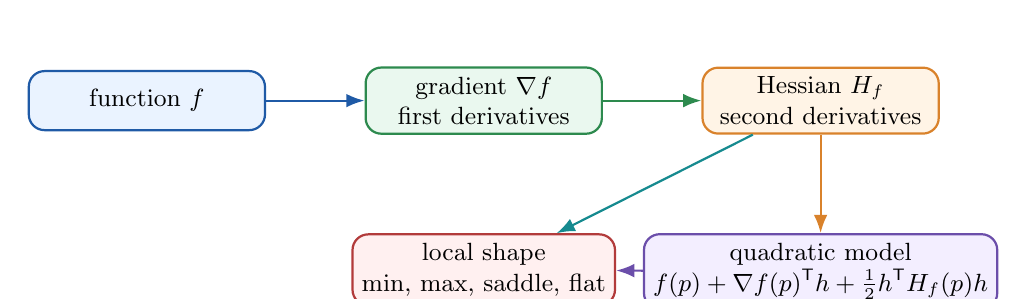
\begin{tikzpicture}[node distance=1.25cm, font=\small]
  \tikzset{box/.style={draw, rounded corners=2mm, thick, align=center, minimum width=3.0cm, minimum height=0.75cm}}
  \node[box, fill=softblue, draw=chapterblue] (f) {function $f$};
  \node[box, fill=softgreen, draw=chaptergreen, right=of f] (g) {gradient $\grad f$\\first derivatives};
  \node[box, fill=softorange, draw=chapterorange, right=of g] (h) {Hessian $H_f$\\second derivatives};
  \node[box, fill=softpurple, draw=chapterpurple, below=of h] (q) {quadratic model\\$f(p)+\grad f(p)\T h+\frac12h\T H_f(p)h$};
  \node[box, fill=softred, draw=chapterred, below=of g] (shape) {local shape\\min, max, saddle, flat};
  \draw[-Latex, thick, chapterblue] (f) -- (g);
  \draw[-Latex, thick, chaptergreen] (g) -- (h);
  \draw[-Latex, thick, chapterorange] (h) -- (q);
  \draw[-Latex, thick, chapterpurple] (q) -- (shape);
  \draw[-Latex, thick, chapterteal] (h) -- (shape);
\end{tikzpicture}
\caption{The flow of second-order thinking: first derivatives build the gradient; second derivatives build the Hessian; the Hessian controls the local quadratic model and local shape.}
\end{figure}

\section{From linear approximation to quadratic approximation}

For a one-variable function, the Taylor approximation at $x=a$ begins as
\[
f(x)\approx f(a)+f'(a)(x-a)+\frac12 f''(a)(x-a)^2.
\]
The first two terms form the tangent-line approximation. The third term adds curvature.

For a two-variable function $f(x,y)$ near $(a,b)$, the linear approximation is
\[
L(x,y)=f(a,b)+f_x(a,b)(x-a)+f_y(a,b)(y-b).
\]
The second-order approximation adds all possible second-order terms:
\[
\begin{aligned}
T_2(x,y)=&\ f(a,b)+f_x(a,b)(x-a)+f_y(a,b)(y-b)\\
&+\frac12 f_{xx}(a,b)(x-a)^2+f_{xy}(a,b)(x-a)(y-b)+\frac12 f_{yy}(a,b)(y-b)^2.
\end{aligned}
\]
The mixed term appears with coefficient $f_{xy}(a,b)$ because the symmetric matrix form contains two equal mixed terms and the factor $1/2$ balances them.

\begin{tipbox}[Compact vector notation]
Let
\[
p=\vect{a\\b},\qquad x=\vect{x\\y},\qquad h=x-p=\vect{x-a\\y-b}.
\]
Then the quadratic Taylor approximation is
\[
f(p+h)\approx f(p)+\grad f(p)\T h+\frac12h\T H_f(p)h.
\]
\end{tipbox}

\begin{figure}[H]
\centering
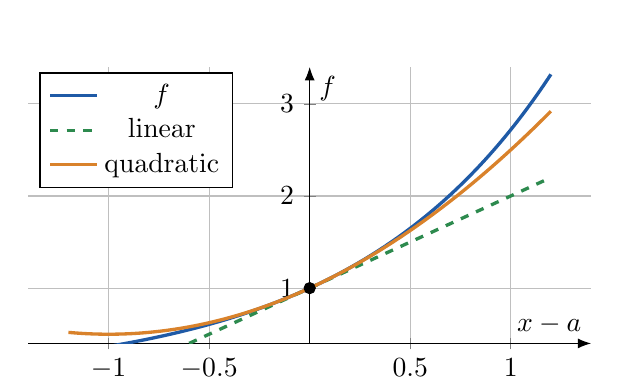
\begin{tikzpicture}
\begin{axis}[
  width=0.72\textwidth,height=0.42\textwidth,
  xmin=-1.4,xmax=1.4,ymin=0.4,ymax=3.4,
  axis lines=middle, xlabel={$x-a$}, ylabel={$f$}, grid=both,
  legend style={at={(0.02,0.98)},anchor=north west,fill=white},
  axis line style={-Latex}
]
\addplot[domain=-1.2:1.2,samples=200,very thick,chapterblue] {exp(x)};
\addlegendentry{$f$}
\addplot[domain=-1.2:1.2,samples=2,very thick,chaptergreen,dashed] {1+x};
\addlegendentry{linear}
\addplot[domain=-1.2:1.2,samples=200,very thick,chapterorange] {1+x+0.5*x^2};
\addlegendentry{quadratic}
\addplot[only marks,mark=*,mark size=2pt] coordinates {(0,1)};
\end{axis}
\end{tikzpicture}
\caption{The one-variable picture: the tangent line gives first-order information; the quadratic approximation adds curvature.}
\end{figure}

\section{The Hessian matrix}

For a function $f(x,y)$ with continuous second partial derivatives, the \textbf{Hessian matrix} is
\[
H_f(x,y)=
\begin{bmatrix}
f_{xx}(x,y) & f_{xy}(x,y)\\
f_{yx}(x,y) & f_{yy}(x,y)
\end{bmatrix}.
\]
When the mixed partial derivatives are continuous, Clairaut's theorem gives $f_{xy}=f_{yx}$, so the Hessian is symmetric.

For $f(x_1,\ldots,x_n)$, the Hessian is the $n\times n$ matrix
\[
H_f(x)=
\begin{bmatrix}
\dfrac{\partial^2 f}{\partial x_1\partial x_1} & \cdots & \dfrac{\partial^2 f}{\partial x_1\partial x_n}\\
\vdots & \ddots & \vdots\\
\dfrac{\partial^2 f}{\partial x_n\partial x_1} & \cdots & \dfrac{\partial^2 f}{\partial x_n\partial x_n}
\end{bmatrix}.
\]
The Hessian is the derivative of the gradient. The gradient tells which direction increases $f$ fastest. The Hessian tells how that gradient changes from point to point.

\begin{figure}[H]
\centering
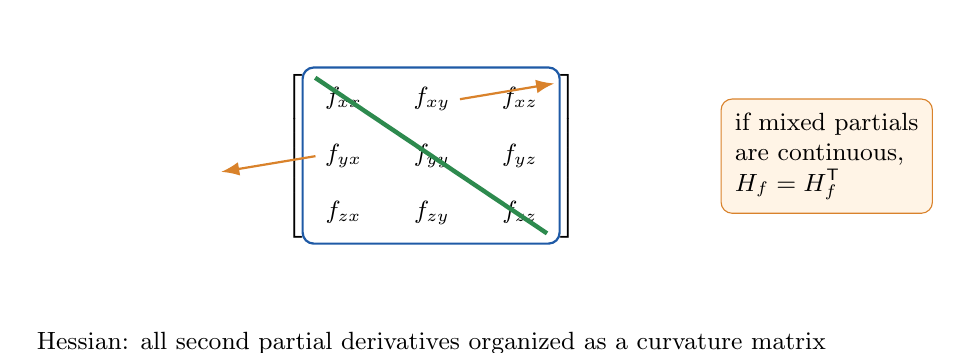
\begin{tikzpicture}[font=\small]
\matrix (M) [matrix of math nodes,left delimiter={[},right delimiter={]},row sep=0.55em,column sep=1.2em] {
f_{xx} & f_{xy} & f_{xz}\\
f_{yx} & f_{yy} & f_{yz}\\
f_{zx} & f_{zy} & f_{zz}\\
};
\draw[chapterblue,thick,rounded corners] ($(M-1-1.north west)+(-0.16,0.13)$) rectangle ($(M-3-3.south east)+(0.16,-0.13)$);
\draw[chaptergreen,ultra thick] (M-1-1.north west) -- (M-3-3.south east);
\node[below=1.0cm of M] {Hessian: all second partial derivatives organized as a curvature matrix};
\node[right=2.2cm of M-2-3, align=left, draw=chapterorange, fill=softorange, rounded corners, inner sep=5pt] {if mixed partials\\are continuous,\\$H_f=H_f\T$};
\draw[-Latex, thick, chapterorange] (M-1-2.east) -- +(1.2,0.2);
\draw[-Latex, thick, chapterorange] (M-2-1.west) -- +(-1.2,-0.2);
\end{tikzpicture}
\caption{The Hessian packages second derivatives into a matrix. Symmetry comes from equality of mixed partial derivatives under standard smoothness assumptions.}
\end{figure}

\section{Worked example: a second-order Taylor polynomial}

\begin{examplebox}{Taylor approximation for $e^{x-y}+xy$}{taylor-example}
Consider
\[
f(x,y)=e^{x-y}+xy.
\]
Find the second-order Taylor approximation at $(0,0)$.

First,
\[
f(0,0)=1,
\qquad
f_x=e^{x-y}+y,
\qquad
f_y=-e^{x-y}+x.
\]
Thus $f_x(0,0)=1$ and $f_y(0,0)=-1$. The second derivatives are
\[
f_{xx}=e^{x-y},\qquad f_{xy}=-e^{x-y}+1,\qquad f_{yy}=e^{x-y}.
\]
At $(0,0)$,
\[
f_{xx}(0,0)=1,\qquad f_{xy}(0,0)=0,\qquad f_{yy}(0,0)=1.
\]
Therefore
\[
T_2(x,y)=1+x-y+\frac12x^2+\frac12y^2.
\]
The first-order terms create a tilted plane. The quadratic terms bend the approximation upward in both coordinate directions.
\end{examplebox}

\begin{figure}[H]
\centering
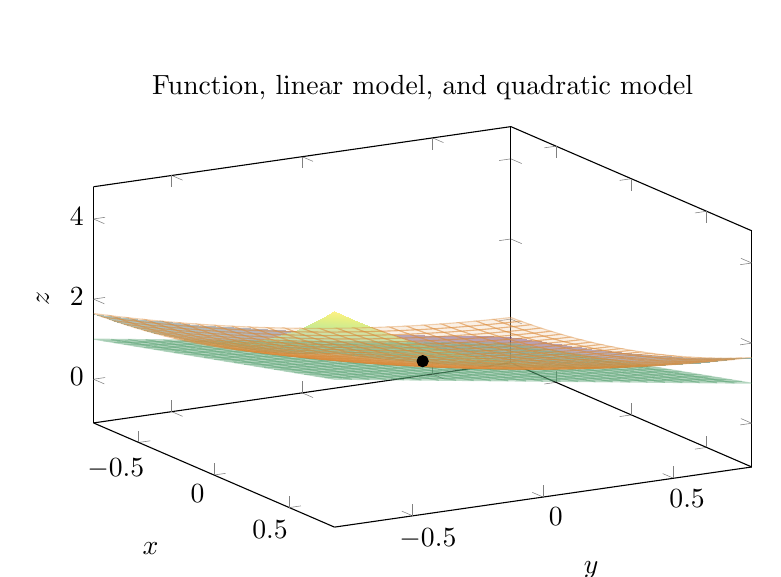
\begin{tikzpicture}
\begin{axis}[
  width=0.82\textwidth,height=0.55\textwidth,
  view={60}{27},xlabel={$x$},ylabel={$y$},zlabel={$z$},
  domain=-0.8:0.8,y domain=-0.8:0.8,samples=25,samples y=25,
  z buffer=sort, title={Function, linear model, and quadratic model}
]
\addplot3[surf,shader=interp,opacity=0.55,colormap/viridis] {exp(x-y)+x*y};
\addplot3[surf,shader=flat,opacity=0.30,draw=chaptergreen,fill=chaptergreen!35] {1+x-y};
\addplot3[surf,shader=flat,opacity=0.35,draw=chapterorange,fill=chapterorange!35] {1+x-y+0.5*x^2+0.5*y^2};
\addplot3[only marks,mark=*,mark size=2pt] coordinates {(0,0,1)};
\end{axis}
\end{tikzpicture}
\caption{Near the expansion point, the quadratic Taylor model follows the true surface more closely than the tangent plane.}
\end{figure}

\section{Quadratic forms}

A \textbf{quadratic form} in two variables has the form
\[
Q(h_1,h_2)=ah_1^2+2bh_1h_2+ch_2^2.
\]
In matrix form,
\[
Q(h)=h\T A h,
\qquad
h=\vect{h_1\\h_2},
\qquad
A=\begin{bmatrix}a&b\\b&c\end{bmatrix}.
\]
The quadratic term in Taylor's formula is exactly a quadratic form:
\[
\frac12h\T H_f(p)h.
\]
Thus local second-order geometry is linear algebra. The shape of a function near a point is controlled by $H_f(p)$.

\begin{figure}[H]
\centering
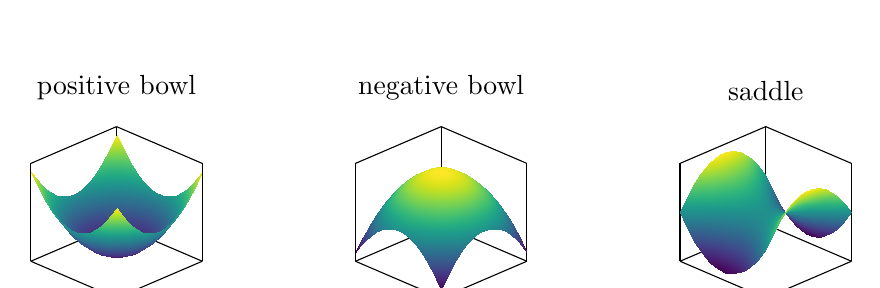
\begin{tikzpicture}
\begin{axis}[width=0.31\textwidth,height=0.31\textwidth,view={45}{28},title={positive bowl},domain=-1.4:1.4,y domain=-1.4:1.4,samples=18,samples y=18,xtick=\empty,ytick=\empty,ztick=\empty]
\addplot3[surf,shader=interp,colormap/viridis] {x^2+y^2};
\end{axis}
\begin{axis}[xshift=0.34\textwidth,width=0.31\textwidth,height=0.31\textwidth,view={45}{28},title={negative bowl},domain=-1.4:1.4,y domain=-1.4:1.4,samples=18,samples y=18,xtick=\empty,ytick=\empty,ztick=\empty]
\addplot3[surf,shader=interp,colormap/viridis] {-x^2-y^2};
\end{axis}
\begin{axis}[xshift=0.68\textwidth,width=0.31\textwidth,height=0.31\textwidth,view={45}{28},title={saddle},domain=-1.4:1.4,y domain=-1.4:1.4,samples=18,samples y=18,xtick=\empty,ytick=\empty,ztick=\empty]
\addplot3[surf,shader=interp,colormap/viridis] {x^2-y^2};
\end{axis}
\end{tikzpicture}
\caption{Three basic quadratic forms: positive definite, negative definite, and indefinite.}
\end{figure}

\section{Definiteness and local shape}

A symmetric matrix $A$ defines a quadratic form $Q(h)=h\T Ah$.
\begin{itemize}
  \item $A$ is \textbf{positive definite} if $h\T Ah>0$ for every nonzero vector $h$.
  \item $A$ is \textbf{negative definite} if $h\T Ah<0$ for every nonzero vector $h$.
  \item $A$ is \textbf{indefinite} if $h\T Ah$ is positive in some directions and negative in others.
  \item $A$ is \textbf{positive semidefinite} if $h\T Ah\ge 0$ for every vector $h$, but may be zero for some nonzero $h$.
  \item $A$ is \textbf{negative semidefinite} if $h\T Ah\le 0$ for every vector $h$, but may be zero for some nonzero $h$.
\end{itemize}

This classification is geometric: positive definite means bowl-shaped, negative definite means upside-down bowl-shaped, indefinite means saddle-shaped, and semidefinite means curved in some directions but flat in others.

\section{Eigenvalues and principal directions}

For a symmetric matrix $A$, the eigenvectors give the principal directions of the quadratic form, and the eigenvalues give the curvature in those directions. If $A$ has orthonormal eigenvectors $u_1,\ldots,u_n$ with eigenvalues $\lambda_1,\ldots,\lambda_n$, and if
\[
h=c_1u_1+\cdots+c_nu_n,
\]
then
\[
h\T Ah=\lambda_1c_1^2+\cdots+\lambda_n c_n^2.
\]
This formula is one of the most important bridges between calculus and linear algebra.

\begin{importantbox}[Hessian eigenvalues and local shape]
At a critical point $p$, the first-order term disappears because $\grad f(p)=0$. Then
\[
f(p+h)-f(p)\approx \frac12h\T H_f(p)h.
\]
Therefore the eigenvalues of $H_f(p)$ determine the local shape:
\begin{itemize}
  \item all positive eigenvalues: local minimum;
  \item all negative eigenvalues: local maximum;
  \item both positive and negative eigenvalues: saddle point;
  \item at least one zero eigenvalue: higher-order analysis may be needed.
\end{itemize}
\end{importantbox}

\begin{figure}[H]
\centering
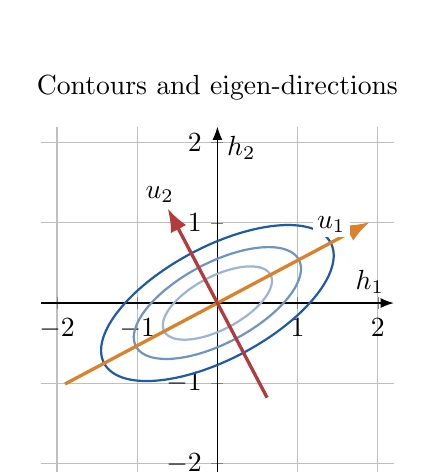
\begin{tikzpicture}
\begin{axis}[
  width=0.62\textwidth,height=0.5\textwidth,
  xmin=-2.2,xmax=2.2,ymin=-2.2,ymax=2.2,axis equal image,
  axis lines=middle,xlabel={$h_1$},ylabel={$h_2$},grid=both,
  axis line style={-Latex},title={Contours and eigen-directions}
]
\addplot[domain=0:360,samples=240,chapterblue,thick] ({1.6*cos(x)*cos(28)-0.7*sin(x)*sin(28)},{1.6*cos(x)*sin(28)+0.7*sin(x)*cos(28)});
\addplot[domain=0:360,samples=240,chapterblue!65,thick] ({1.15*cos(x)*cos(28)-0.50*sin(x)*sin(28)},{1.15*cos(x)*sin(28)+0.50*sin(x)*cos(28)});
\addplot[domain=0:360,samples=240,chapterblue!45,thick] ({0.75*cos(x)*cos(28)-0.33*sin(x)*sin(28)},{0.75*cos(x)*sin(28)+0.33*sin(x)*cos(28)});
\addplot[chapterorange,very thick,-Latex] coordinates {(-1.9,-1.01) (1.9,1.01)};
\addplot[chapterred,very thick,-Latex] coordinates {(0.62,-1.18) (-0.62,1.18)};
\node[fill=white,inner sep=1.5pt] at (axis cs:1.42,0.98) {$u_1$};
\node[fill=white,inner sep=1.5pt] at (axis cs:-0.72,1.35) {$u_2$};
\end{axis}
\end{tikzpicture}
\caption{For a symmetric Hessian, eigenvectors give principal axes of the contour ellipses and eigenvalues give curvature along those axes.}
\end{figure}

\section{The two-variable determinant test revisited}

For a two-variable function at a critical point $(a,b)$,
\[
H_f(a,b)=\begin{bmatrix}f_{xx}(a,b)&f_{xy}(a,b)\\f_{xy}(a,b)&f_{yy}(a,b)\end{bmatrix}.
\]
Let
\[
D=f_{xx}(a,b)f_{yy}(a,b)-\bigl(f_{xy}(a,b)\bigr)^2.
\]
The determinant test is a convenient two-variable version of the eigenvalue test:
\begin{itemize}
  \item If $D>0$ and $f_{xx}(a,b)>0$, then $H_f(a,b)$ is positive definite and $f$ has a local minimum.
  \item If $D>0$ and $f_{xx}(a,b)<0$, then $H_f(a,b)$ is negative definite and $f$ has a local maximum.
  \item If $D<0$, then $H_f(a,b)$ is indefinite and $f$ has a saddle point.
  \item If $D=0$, the test is inconclusive.
\end{itemize}
The determinant measures whether the two eigenvalues have the same sign or opposite signs. The entry $f_{xx}$ then tells whether the same sign is positive or negative.

\begin{figure}[H]
\centering
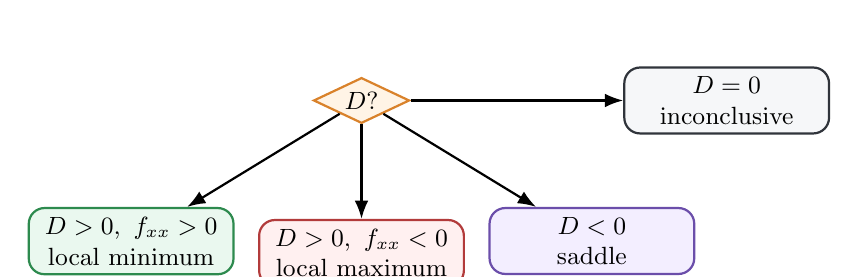
\begin{tikzpicture}[font=\small,node distance=1.0cm]
  \tikzset{decision/.style={diamond, draw, thick, aspect=2.1, align=center, inner sep=1.5pt, fill=softorange}, result/.style={draw, thick, rounded corners=2mm, align=center, minimum width=2.6cm, minimum height=0.7cm}}
  \node[decision, draw=chapterorange] (D) {$D$?};
  \node[result, fill=softgreen, draw=chaptergreen, below left=1.2cm and 1.3cm of D] (min) {$D>0,\ f_{xx}>0$\\local minimum};
  \node[result, fill=softred, draw=chapterred, below=1.2cm of D] (max) {$D>0,\ f_{xx}<0$\\local maximum};
  \node[result, fill=softpurple, draw=chapterpurple, below right=1.2cm and 1.3cm of D] (sad) {$D<0$\\saddle};
  \node[result, fill=softgray, draw=darkgray, right=2.7cm of D] (inc) {$D=0$\\inconclusive};
  \draw[-Latex, thick] (D) -- (min);
  \draw[-Latex, thick] (D) -- (max);
  \draw[-Latex, thick] (D) -- (sad);
  \draw[-Latex, thick] (D) -- (inc);
\end{tikzpicture}
\caption{The determinant test is a quick way to read the two eigenvalue signs of a $2\times2$ Hessian.}
\end{figure}

\section{Worked example: classify critical points}

\begin{examplebox}{Classifying critical points by quadratic approximation}{classify-critical}
Let
\[
f(x,y)=x^3+y^3-3xy+4.
\]
The gradient is
\[
f_x=3x^2-3y,
\qquad
f_y=3y^2-3x.
\]
Critical points satisfy $y=x^2$ and $x=y^2$. Hence $x=x^4$, so $x=0$ or $x=1$. The critical points are $(0,0)$ and $(1,1)$.

The Hessian is
\[
H_f(x,y)=\begin{bmatrix}6x&-3\\-3&6y\end{bmatrix}.
\]
At $(0,0)$,
\[
H_f(0,0)=\begin{bmatrix}0&-3\\-3&0\end{bmatrix},
\qquad D=-9<0,
\]
so $(0,0)$ is a saddle point. At $(1,1)$,
\[
H_f(1,1)=\begin{bmatrix}6&-3\\-3&6\end{bmatrix},
\qquad D=27>0,
\qquad f_{xx}(1,1)=6>0,
\]
so $(1,1)$ is a local minimum, with value $f(1,1)=3$.
\end{examplebox}

\begin{figure}[H]
\centering
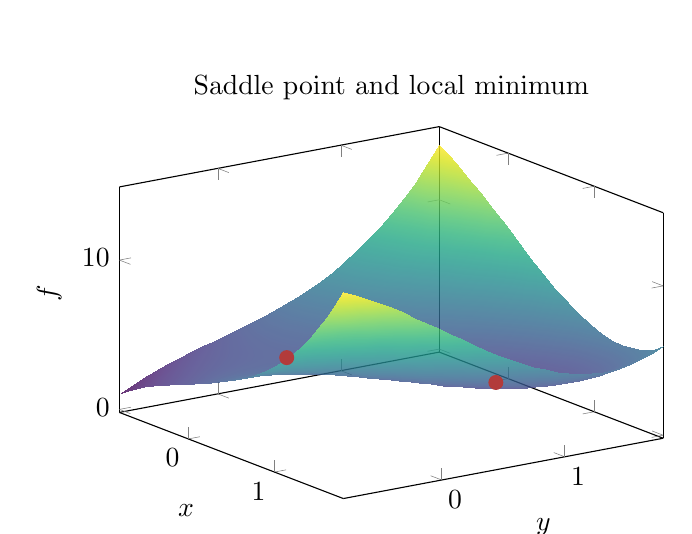
\begin{tikzpicture}
\begin{axis}[
  width=0.7\textwidth,height=0.52\textwidth,
  view={55}{25},xlabel={$x$},ylabel={$y$},zlabel={$f$},
  domain=-0.8:1.8,y domain=-0.8:1.8,samples=28,samples y=28,
  z buffer=sort,title={Saddle point and local minimum}
]
\addplot3[surf,shader=interp,opacity=0.8,colormap/viridis] {x^3+y^3-3*x*y+4};
\addplot3[only marks,mark=*,mark size=2.5pt,chapterred] coordinates {(0,0,4) (1,1,3)};
\end{axis}
\end{tikzpicture}
\caption{Near a critical point, the quadratic Taylor approximation predicts whether the surface behaves like a saddle or a bowl.}
\end{figure}

\section{Taylor approximation in $\R^n$}

For $f:\R^n\to\R$, the second-order Taylor approximation near $p$ is
\[
f(p+h)\approx f(p)+\grad f(p)\T h+\frac12h\T H_f(p)h.
\]
This formula is independent of dimension. The only difference is that $h$ has $n$ components and $H_f(p)$ is an $n\times n$ matrix.

A useful way to read the formula is
\[
\text{new value}\approx \text{base value}+\text{linear change}+\text{curvature correction}.
\]
The first-order term dominates for very small $h$ unless $\grad f(p)=0$. At a critical point, the quadratic term becomes the leading term.

\begin{examplebox}{Second-order approximation in three variables}{three-variable}
Let
\[
f(x,y,z)=x^2+2y^2+3z^2+xy-yz+2x.
\]
At $p=(0,0,0)$,
\[
f(p)=0,
\qquad
\grad f(p)=\vect{2\\0\\0}.
\]
The Hessian is constant:
\[
H_f=\begin{bmatrix}2&1&0\\1&4&-1\\0&-1&6\end{bmatrix}.
\]
For $h=(h_1,h_2,h_3)\T$,
\[
f(h)=2h_1+\frac12h\T H_fh.
\]
The Taylor approximation is exact because $f$ is already a quadratic polynomial plus a linear term.
\end{examplebox}

\begin{figure}[H]
\centering
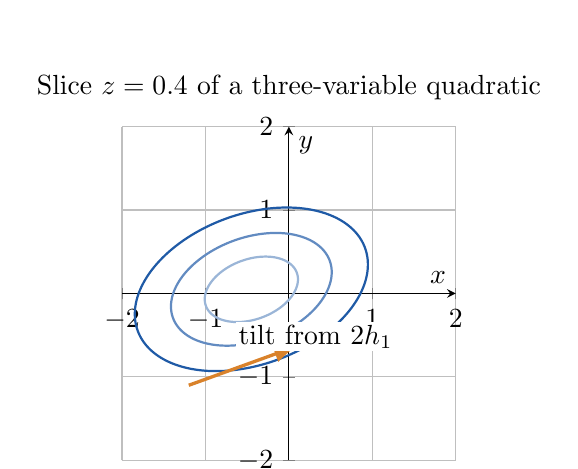
\begin{tikzpicture}
\begin{axis}[
  width=0.66\textwidth,height=0.48\textwidth,
  xmin=-2,xmax=2,ymin=-2,ymax=2,axis equal image,
  axis lines=middle,xlabel={$x$},ylabel={$y$},grid=both,
  title={Slice $z=0.4$ of a three-variable quadratic}
]
\addplot[domain=0:360,samples=200,chapterblue,thick] ({1.45*cos(x)*cos(20)-0.9*sin(x)*sin(20)-0.45},{1.45*cos(x)*sin(20)+0.9*sin(x)*cos(20)+0.05});
\addplot[domain=0:360,samples=200,chapterblue!70,thick] ({1.0*cos(x)*cos(20)-0.62*sin(x)*sin(20)-0.45},{1.0*cos(x)*sin(20)+0.62*sin(x)*cos(20)+0.05});
\addplot[domain=0:360,samples=200,chapterblue!45,thick] ({0.58*cos(x)*cos(20)-0.36*sin(x)*sin(20)-0.45},{0.58*cos(x)*sin(20)+0.36*sin(x)*cos(20)+0.05});
\addplot[chapterorange,very thick,-Latex] coordinates {(-1.2,-1.1) (0.1,-0.63)};
\node[fill=white,inner sep=1pt] at (axis cs:0.32,-0.52) {tilt from $2h_1$};
\end{axis}
\end{tikzpicture}
\caption{A two-dimensional slice of a three-variable quadratic model: contours reveal curvature and the linear term tilts the landscape.}
\end{figure}

\section{Least squares as a quadratic form}

Second-order geometry is especially clear in least squares. Suppose $X$ is a data matrix, $y$ is a response vector, and $\beta$ is a parameter vector. The least-squares loss is
\[
L(\beta)=\norm{y-X\beta}^2.
\]
Expanding,
\[
L(\beta)=y\T y-2\beta\T X\T y+\beta\T X\T X\beta.
\]
This is a quadratic function of $\beta$. Its gradient is
\[
\grad L(\beta)=2X\T(X\beta-y),
\]
and its Hessian is
\[
H_L(\beta)=2X\T X.
\]
The Hessian does not depend on $\beta$. The eigenvalues of $2X\T X$ determine the shape of the loss landscape: large eigenvalues mean steep curvature, small eigenvalues mean flat directions, and zero eigenvalues mean non-unique least-squares solutions.

\begin{figure}[H]
\centering
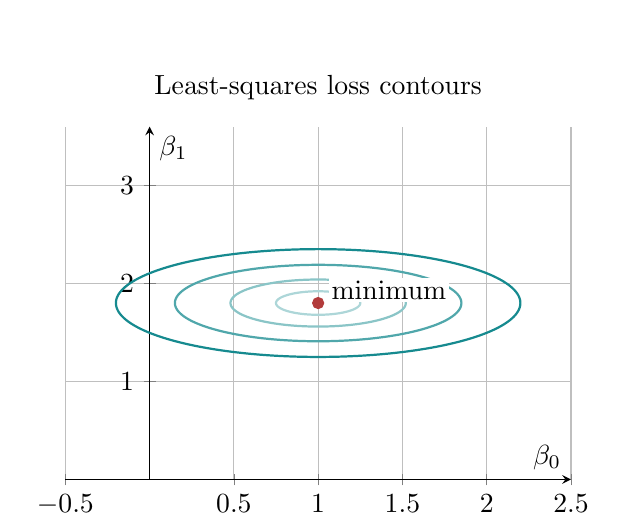
\begin{tikzpicture}
\begin{axis}[
  width=0.66\textwidth,height=0.50\textwidth,
  xmin=-0.5,xmax=2.5,ymin=0,ymax=3.6,
  axis lines=middle,xlabel={$\beta_0$},ylabel={$\beta_1$},grid=both,
  title={Least-squares loss contours}
]
\addplot[domain=0:360,samples=220,chapterteal,thick] ({1.0+1.20*cos(x)},{1.8+0.55*sin(x)});
\addplot[domain=0:360,samples=220,chapterteal!75,thick] ({1.0+0.85*cos(x)},{1.8+0.39*sin(x)});
\addplot[domain=0:360,samples=220,chapterteal!50,thick] ({1.0+0.52*cos(x)},{1.8+0.24*sin(x)});
\addplot[domain=0:360,samples=220,chapterteal!35,thick] ({1.0+0.25*cos(x)},{1.8+0.12*sin(x)});
\addplot[only marks,mark=*,mark size=2pt,chapterred] coordinates {(1.0,1.8)};
\node[fill=white,inner sep=1pt] at (axis cs:1.42,1.93) {minimum};
\end{axis}
\end{tikzpicture}
\caption{A least-squares loss is a quadratic surface in the model parameters; its contours are ellipses when the Hessian is positive definite.}
\end{figure}

\section{Newton's method from Taylor approximation}

Second-order Taylor approximation also explains Newton's method for optimization. Suppose $f:\R^n\to\R$ is smooth and we are at $x_k$. Let $h$ be a small step. The quadratic model is
\[
m_k(h)=f(x_k)+\grad f(x_k)\T h+\frac12h\T H_f(x_k)h.
\]
To minimize this quadratic model, set its gradient with respect to $h$ equal to zero:
\[
\grad f(x_k)+H_f(x_k)h=0.
\]
Thus the Newton step satisfies
\[
H_f(x_k)h=-\grad f(x_k),
\qquad
x_{k+1}=x_k+h.
\]
When the Hessian is positive definite and the starting point is close enough to a local minimum, Newton's method can converge very quickly. When the Hessian is indefinite or nearly singular, the Newton step may point toward a saddle or become unstable.

\begin{figure}[H]
\centering
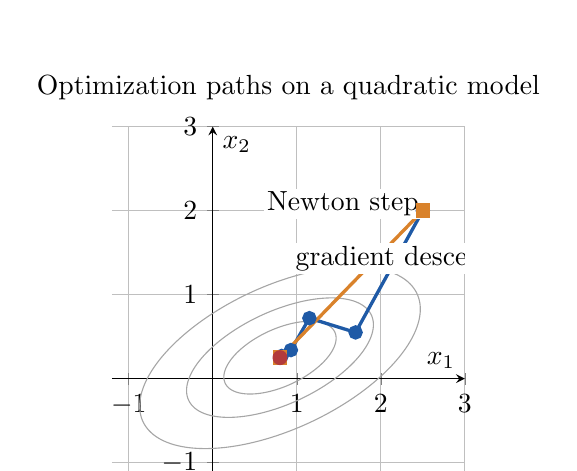
\begin{tikzpicture}
\begin{axis}[
  width=0.64\textwidth,height=0.50\textwidth,
  xmin=-1.2,xmax=3.0,ymin=-1.2,ymax=3.0,
  axis equal image,axis lines=middle,xlabel={$x_1$},ylabel={$x_2$},grid=both,
  title={Optimization paths on a quadratic model}
]
\addplot[domain=0:360,samples=220,gray!70] ({0.8+1.8*cos(x)*cos(25)-0.85*sin(x)*sin(25)},{0.25+1.8*cos(x)*sin(25)+0.85*sin(x)*cos(25)});
\addplot[domain=0:360,samples=220,gray!70] ({0.8+1.2*cos(x)*cos(25)-0.55*sin(x)*sin(25)},{0.25+1.2*cos(x)*sin(25)+0.55*sin(x)*cos(25)});
\addplot[domain=0:360,samples=220,gray!70] ({0.8+0.72*cos(x)*cos(25)-0.34*sin(x)*sin(25)},{0.25+0.72*cos(x)*sin(25)+0.34*sin(x)*cos(25)});
\addplot[chapterblue,very thick,mark=*] coordinates {(2.5,2.0) (1.7,0.55) (1.15,0.72) (0.93,0.34) (0.82,0.27)};
\addplot[chapterorange,very thick,mark=square*] coordinates {(2.5,2.0) (0.8,0.25)};
\addplot[only marks,mark=*,mark size=2.5pt,chapterred] coordinates {(0.8,0.25)};
\node[fill=white,inner sep=1pt] at (axis cs:2.16,1.43) {gradient descent};
\node[fill=white,inner sep=1pt] at (axis cs:1.55,2.08) {Newton step};
\end{axis}
\end{tikzpicture}
\caption{On a quadratic model, Newton's step jumps to the minimizer in one exact step, while gradient descent follows the negative-gradient direction repeatedly.}
\end{figure}

\section{Conditioning and narrow valleys}

A positive definite Hessian may still create numerical difficulty. If the eigenvalues of $H$ have very different sizes, then the quadratic bowl is narrow and stretched. The ratio
\[
\kappa(H)=\frac{\lambda_{\max}}{\lambda_{\min}}
\]
is the \textbf{condition number} of the Hessian when all eigenvalues are positive.

A large condition number means the function is much steeper in one direction than another. Gradient descent may zigzag in narrow valleys. Newton's method corrects for curvature by multiplying by $H^{-1}$, but this can be expensive or unstable in high dimensions.

\begin{figure}[H]
\centering
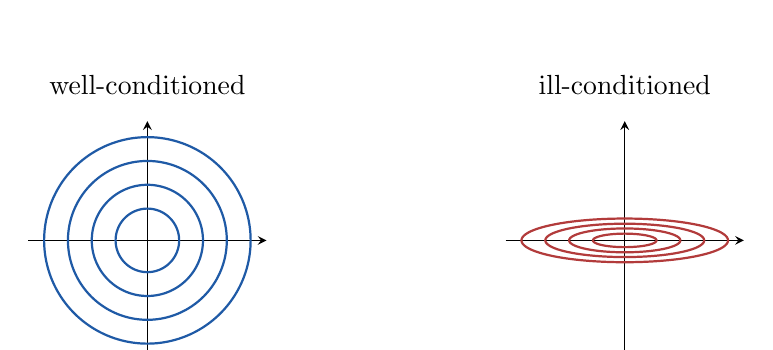
\begin{tikzpicture}
\begin{axis}[width=0.45\textwidth,height=0.38\textwidth,xmin=-3,xmax=3,ymin=-3,ymax=3,axis equal image,axis lines=middle,title={well-conditioned},xtick=\empty,ytick=\empty]
\foreach \r in {0.8,1.4,2.0,2.6}{\addplot[domain=0:360,samples=180,chapterblue,thick] ({\r*cos(x)},{\r*sin(x)});}
\end{axis}
\begin{axis}[xshift=0.50\textwidth,width=0.45\textwidth,height=0.38\textwidth,xmin=-3,xmax=3,ymin=-3,ymax=3,axis equal image,axis lines=middle,title={ill-conditioned},xtick=\empty,ytick=\empty]
\foreach \a/\b in {2.6/0.55,2.0/0.42,1.4/0.30,0.8/0.17}{\addplot[domain=0:360,samples=180,chapterred,thick] ({\a*cos(x)},{\b*sin(x)});}
\end{axis}
\end{tikzpicture}
\caption{A large Hessian condition number produces narrow, stretched contours; this is a geometric source of slow gradient descent.}
\end{figure}

\section{Statistical interpretation: likelihood and uncertainty}

In statistics, second-order approximation appears in the local behavior of a log-likelihood. Suppose $\ell(\theta)$ is a log-likelihood and $\hat\theta$ is a maximum likelihood estimate. Since $\hat\theta$ is a critical point,
\[
\grad \ell(\hat\theta)=0.
\]
The second-order Taylor approximation is
\[
\ell(\theta)\approx \ell(\hat\theta)+\frac12(\theta-\hat\theta)\T H_\ell(\hat\theta)(\theta-\hat\theta).
\]
At a local maximum, the Hessian is negative definite. The negative Hessian
\[
-H_\ell(\hat\theta)
\]
measures local curvature of the log-likelihood. Sharper curvature means the likelihood drops quickly away from the estimate, indicating smaller uncertainty. Flatter curvature means larger uncertainty.

\begin{figure}[H]
\centering
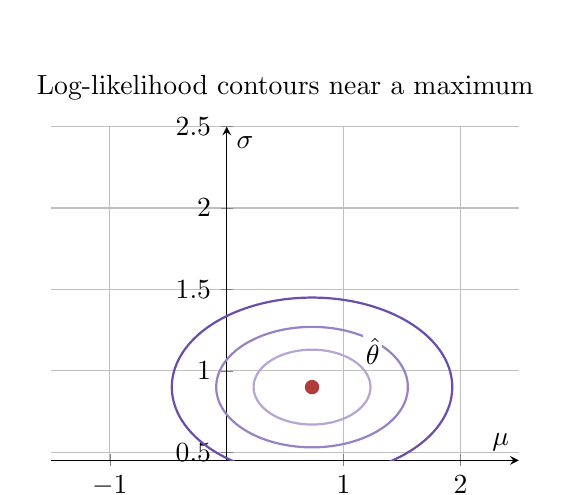
\begin{tikzpicture}
\begin{axis}[
  width=0.62\textwidth,height=0.48\textwidth,
  xmin=-1.5,xmax=2.5,ymin=0.45,ymax=2.5,
  axis lines=middle,xlabel={$\mu$},ylabel={$\sigma$},grid=both,
  title={Log-likelihood contours near a maximum}
]
\addplot[domain=0:360,samples=220,chapterpurple,thick] ({0.73+1.2*cos(x)},{0.45+0.55*sin(x)+0.45});
\addplot[domain=0:360,samples=220,chapterpurple!70,thick] ({0.73+0.82*cos(x)},{0.90+0.37*sin(x)});
\addplot[domain=0:360,samples=220,chapterpurple!50,thick] ({0.73+0.50*cos(x)},{0.90+0.23*sin(x)});
\addplot[only marks,mark=*,mark size=2.4pt,chapterred] coordinates {(0.73,0.90)};
\node[fill=white,inner sep=1pt] at (axis cs:1.25,1.12) {$\hat\theta$};
\end{axis}
\end{tikzpicture}
\caption{Near a maximum, a smooth log-likelihood is often well approximated by a concave quadratic. The negative Hessian describes local precision.}
\end{figure}

\section{Beyond second order and degenerate examples}

The second-order Taylor approximation is powerful, but it has limitations:
\begin{enumerate}
  \item If the Hessian is singular, second-order information may not classify a critical point.
  \item If the point is far from the center of approximation, higher-order terms may dominate.
  \item If the function is not twice continuously differentiable, the Hessian may not describe local geometry reliably.
  \item In high-dimensional models, the Hessian may be too large to store or invert directly.
\end{enumerate}

The function $f(x,y)=x^4+y^4$ has a local minimum at $(0,0)$, but its Hessian at the origin is the zero matrix. The second derivative test gives no information, even though the function is clearly nonnegative. The function $g(x,y)=x^4-y^4$ also has zero Hessian at the origin, but the origin is a saddle point. When the Hessian is degenerate, higher-order terms matter.

\begin{figure}[H]
\centering
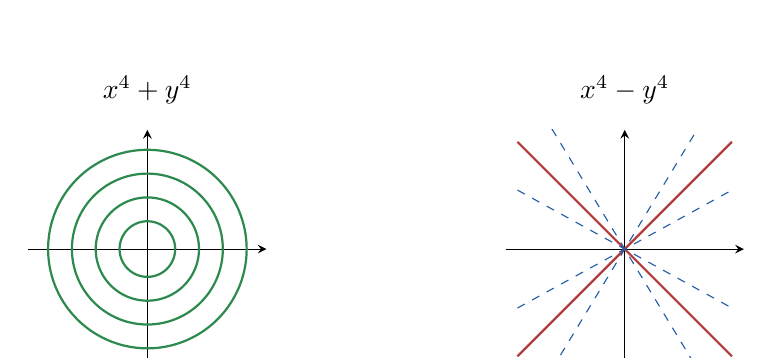
\begin{tikzpicture}
\begin{axis}[width=0.45\textwidth,height=0.38\textwidth,xmin=-1.5,xmax=1.5,ymin=-1.5,ymax=1.5,axis equal image,axis lines=middle,title={$x^4+y^4$},xtick=\empty,ytick=\empty]
\foreach \r in {0.35,0.65,0.95,1.25}{\addplot[domain=0:360,samples=180,chaptergreen,thick] ({\r*cos(x)},{\r*sin(x)});}
\end{axis}
\begin{axis}[xshift=0.50\textwidth,width=0.45\textwidth,height=0.38\textwidth,xmin=-1.5,xmax=1.5,ymin=-1.5,ymax=1.5,axis equal image,axis lines=middle,title={$x^4-y^4$},xtick=\empty,ytick=\empty]
\addplot[domain=-1.35:1.35,samples=160,chapterred,thick] {x};
\addplot[domain=-1.35:1.35,samples=160,chapterred,thick] {-x};
\addplot[domain=-1.35:1.35,samples=160,chapterblue,dashed] {0.55*x};
\addplot[domain=-1.35:1.35,samples=160,chapterblue,dashed] {-0.55*x};
\addplot[domain=-1.35:1.35,samples=160,chapterblue,dashed] {1.65*x};
\addplot[domain=-1.35:1.35,samples=160,chapterblue,dashed] {-1.65*x};
\end{axis}
\end{tikzpicture}
\caption{Degenerate critical points may require higher-order terms beyond the Hessian. Both examples have zero Hessian at the origin, but their local behavior is different.}
\end{figure}

\section{Algorithmic summary}

To use second-order approximation in practice:
\begin{enumerate}
  \item Choose a center point $p$.
  \item Compute $f(p)$, $\grad f(p)$, and $H_f(p)$.
  \item Form the local model
  \[
  T_2(p+h)=f(p)+\grad f(p)\T h+\frac12h\T H_f(p)h.
  \]
  \item At a critical point, classify the Hessian using eigenvalues or definiteness tests.
  \item Interpret the eigenvectors as principal directions and eigenvalues as curvatures.
  \item Use the approximation only locally unless the function is exactly quadratic.
\end{enumerate}

\begin{figure}[H]
\centering
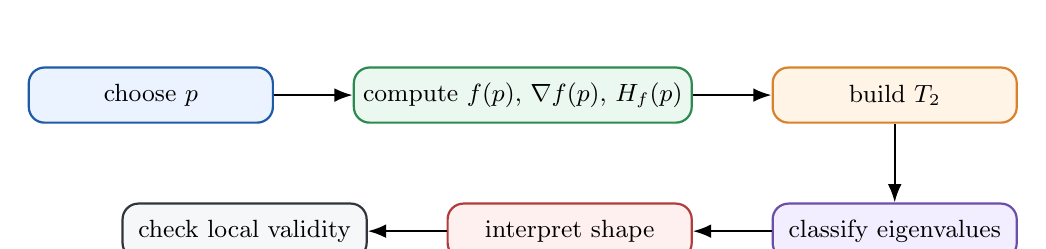
\begin{tikzpicture}[font=\small,node distance=1.0cm]
  \tikzset{flowstep/.style={draw, thick, rounded corners=2mm, fill=softblue, align=center, minimum width=3.1cm, minimum height=0.7cm}}
  \node[flowstep, draw=chapterblue] (s1) {choose $p$};
  \node[flowstep, draw=chaptergreen, right=of s1, fill=softgreen] (s2) {compute $f(p)$, $\grad f(p)$, $H_f(p)$};
  \node[flowstep, draw=chapterorange, right=of s2, fill=softorange] (s3) {build $T_2$};
  \node[flowstep, draw=chapterpurple, below=of s3, fill=softpurple] (s4) {classify eigenvalues};
  \node[flowstep, draw=chapterred, left=of s4, fill=softred] (s5) {interpret shape};
  \node[flowstep, draw=darkgray, left=of s5, fill=softgray] (s6) {check local validity};
  \draw[-Latex, thick] (s1) -- (s2);
  \draw[-Latex, thick] (s2) -- (s3);
  \draw[-Latex, thick] (s3) -- (s4);
  \draw[-Latex, thick] (s4) -- (s5);
  \draw[-Latex, thick] (s5) -- (s6);
\end{tikzpicture}
\caption{A practical workflow for second-order approximation and Hessian-based classification.}
\end{figure}

\section{Python lab preview}

The companion notebook for this chapter asks students to build a small second-order approximation toolkit:
\begin{itemize}
  \item input a symbolic or numerical function;
  \item compute or approximate the gradient;
  \item compute or approximate the Hessian;
  \item build a quadratic Taylor model;
  \item plot the true function and approximation;
  \item classify a critical point by Hessian eigenvalues.
\end{itemize}

A finite-difference Hessian can approximate local curvature when symbolic derivatives are unavailable. For a numerical function $f:\R^n\to\R$, the central-difference formula
\[
H_{ij}(p)\approx
\frac{f(p+\varepsilon e_i+\varepsilon e_j)-f(p+\varepsilon e_i-\varepsilon e_j)-f(p-\varepsilon e_i+\varepsilon e_j)+f(p-\varepsilon e_i-\varepsilon e_j)}{4\varepsilon^2}
\]
provides an approximation to the $(i,j)$ entry of the Hessian.

\section{Exercises}

\subsection*{Conceptual questions}
\begin{enumerate}
  \item Explain the difference between a linear approximation and a quadratic approximation.
  \item What does the Hessian matrix measure that the gradient does not measure?
  \item Why does the quadratic term dominate the local shape at a critical point?
  \item Explain why a positive definite Hessian produces a local minimum.
  \item Explain why an indefinite Hessian produces a saddle point.
  \item What does it mean geometrically for a Hessian to have a zero eigenvalue?
  \item Why are eigenvectors of the Hessian called principal directions?
  \item In least squares, why is the loss function quadratic in the parameters?
  \item Why can Newton's method be faster than gradient descent near a well-conditioned minimum?
  \item Why can a degenerate critical point require higher-order Taylor terms?
\end{enumerate}

\subsection*{Computational practice}
\begin{enumerate}[start=11]
  \item Find the second-order Taylor approximation of $f(x,y)=\sin(x+y)$ at $(0,0)$.
  \item Find the second-order Taylor approximation of $f(x,y)=e^x\cos y$ at $(0,0)$.
  \item Find the Hessian of $f(x,y)=x^2+4xy+3y^2$ and classify its quadratic form.
  \item Find the Hessian of $f(x,y)=x^2-y^2+2xy$ and classify its quadratic form.
  \item For $f(x,y)=x^3+y^3-3xy+4$, verify all critical points and classify them.
  \item For $f(x,y)=x^4+y^4-4xy$, find all critical points and use the Hessian test where possible.
  \item Let $f(x,y,z)=x^2+2y^2+3z^2+xy-yz$. Compute $H_f$ and its eigenvalues.
  \item Let $A=\begin{bmatrix}5&2\\2&2\end{bmatrix}$. Determine whether $h\T Ah$ is positive definite.
  \item Let $A=\begin{bmatrix}1&3\\3&1\end{bmatrix}$. Determine whether $h\T Ah$ is positive definite, negative definite, or indefinite.
  \item Show that if $A=X\T X$, then $A$ is positive semidefinite.
\end{enumerate}

\subsection*{Applications and modeling}
\begin{enumerate}[start=21]
  \item For the least-squares loss $L(\beta)=\norm{y-X\beta}^2$, derive the gradient and Hessian.
  \item Explain how the eigenvalues of $X\T X$ affect gradient descent for least squares.
  \item Suppose a log-likelihood has Hessian $\begin{bmatrix}-10&0\\0&-1\end{bmatrix}$ at its maximum. Which parameter direction is more uncertain?
  \item For a two-parameter model, design a quadratic loss with a narrow valley and plot its contours.
  \item Implement a finite-difference Hessian for a function of two variables and test it on $f(x,y)=e^{x-y}+xy$.
\end{enumerate}

\subsection*{Challenge problems}
\begin{enumerate}[start=26]
  \item Show that if all eigenvalues of a symmetric Hessian at a critical point are positive, then the critical point is a strict local minimum.
  \item Give an example where the Hessian test is inconclusive but the critical point is a local minimum.
  \item Give an example where the Hessian test is inconclusive but the critical point is a saddle point.
  \item Let $f(x,y)=x^2+2cxy+y^2$. For which values of $c$ is the origin a local minimum?
  \item Let $f(x,y)=x^2+2cxy+4y^2$. For which values of $c$ is the Hessian positive definite?
\end{enumerate}

\section{Chapter summary}

Second-order Taylor approximation extends tangent-plane approximation by adding curvature. In several variables, curvature is encoded by the Hessian matrix. The quadratic term
\[
\frac12h\T H_f(p)h
\]
is a quadratic form, so the local geometry of a function is controlled by linear algebra. At a critical point, the gradient term disappears and the Hessian determines whether the function locally behaves like a bowl, an upside-down bowl, a saddle, or a degenerate flat shape.

This chapter is a bridge from calculus to modern applied mathematics. Quadratic approximations explain second derivative tests, Newton's method, least-squares geometry, local likelihood approximations, uncertainty quantification, and the curvature of loss landscapes.

\section{Python lab and interactive page}
\begin{notebox}[Companion resources]
The companion resources are the Chapter 18 notebook lab and the Chapter 18 interactive HTML page in the book repository.
\end{notebox}

\end{document}
